\let\lesson\undefined
\newcommand{\lesson}{\phantomlesson{Bài 11.}}
\setcounter{section}{2}
\section{Bài tập trắc nghiệm}
\begin{enumerate}[label=\bfseries Câu \arabic*:]
	\item \mkstar{2}\\
	{Điều nào sau đây đúng khi nói về lực cản tác dụng lên một vật chuyển động trong chất lưu?
		\begin{mcq}
			\item Lực cản của chất lưu cùng phương cùng chiều với chiều chuyển động của vật.
			\item Lực cản của chất lưu không phụ thuộc vào hình dạng của vật.
			\item Lực cản của chất lưu tăng khi tốc độ của vật tăng và không đổi khi vật chuyển động đạt tốc độ tới hạn.
			\item Lực cản của chất lưu càng lớn khi vật có khối lượng càng lớn.
		\end{mcq}
	
}
\hideall{
\textbf{Đáp án: C.}
}

\item \mkstar{2}\\
{Lực đẩy Archimedes phụ thuộc vào các yếu tố
	\begin{mcq}
		\item Trọng lượng riêng của vật và thể tích của phần chất lỏng bị vật chiếm chỗ.
		\item Trọng lượng riêng của chất lỏng và thể tích của vật.
		\item Trọng lượng của vật và thể tích của phần chất lỏng bị vật chiếm chỗ.
		\item Trọng lượng riêng của chất lỏng và thể tích của phần chất lỏng bị vật chiếm chỗ.
	\end{mcq}

}
\hideall{
\textbf{Đáp án: D.}
}

\item \mkstar{2}\\
{Một thỏi nhôm đặc và một thỏi thép đặc có thể tích bằng nhau cùng được nhúng chìm trong nước. Nhận xét nào sau đây là đúng?
	\begin{mcq}
		\item Thỏi nào chìm sâu hơn thì lực đẩy Archimedes tác dụng lên thỏi đó lớn hơn.
		\item Thép có trọng lượng riêng lớn hơn nhôm nên thỏi thép chịu tác dụng của lực đẩy Archimedes lớn hơn.
		\item Hai thỏi nhôm và thép đều chịu tác dụng của lực đẩy Archimedes như nhau vì chúng cùng được nhúng trong nước như nhau.
		\item Hai thỏi nhôm và thép đều chịu tác dụng của lực đẩy Archimedes như nhau vì chúng chiếm thể tích trong nước như nhau.
	\end{mcq}

}
\hideall{
\textbf{Đáp án: D.}
}

\item\mkstar{2}\\
{Lực đẩy Archimedes tác dụng lên một vật nhúng trong chất lỏng bằng
	\begin{mcq}(2)
		\item trọng lượng của vật.
		\item trọng lượng của chất lỏng.
		\item trọng lượng phần chất lỏng bị vật chiếm chỗ.
		\item trọng lượng của phần vật nằm dưới mặt chất lỏng.
	\end{mcq}

}
\hideall{
\textbf{Đáp án: B.}
}

\item\mkstar{2}\\
{Khi nâng một tảng đá ở trong nước ta thấy nhẹ hơn khi nâng nó trong không khí. Sở dĩ như vậy là vì
	\begin{mcq}(2)
		\item khối lượng của tảng đá thay đổi.
		\item khối lượng của nước thay đổi.
		\item lực nâng của nước tác dụng lên hòn đá.
		\item lực đẩy của tảng đá.
	\end{mcq}

}
\hideall{
\textbf{Đáp án: C.}
}

\item \mkstar{2}\\
{Ta biết công thức tính lực đẩy Archimedes là $F_A=\rho gV$ . Ở hình vẽ bên thì $V$ là thể tích nào?
	\begin{center}
		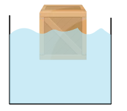
\includegraphics[width=0.15\linewidth]{../figs/VN10-2022-PH-TP020-P-1}
	\end{center}
\begin{mcq}(2)
	\item Thể tích toàn bộ vật.
	\item Thể tích toàn bộ chất lỏng.
	\item Thể tích phần chìm của vật.
	\item Thể tích phần nổi của vật.
\end{mcq}
}
\hideall{
\textbf{Đáp án: C.}
}

\item\mkstar{3}\\
{Một quả cầu bằng sắt có thể tích $\SI{4}{\deci\meter^3}$ được nhúng chìm trong nước, biết khối lượng riêng của nước $\SI{1000}{\kilogram/\meter^3}$. Lực đẩy Archimedes tác dụng lên quả cầu là
	\begin{mcq}(4)
		\item $\SI{4000}{\newton}$.
		\item $\SI{40000}{\newton}$.
		\item $\SI{2500}{\newton}$.
		\item $\SI{40}{\newton}$.
	\end{mcq}

}
\hideall{
\textbf{Đáp án: D.}
}

\item \mkstar{3}\\
{Một quả cầu bằng sắt treo vào 1 lực kế ở ngoài không khí lực kế chỉ $\SI{1.7}{\newton}$. Nhúng chìm quả cầu vào nước thì lực kế chỉ $\SI{1.2}{\newton}$. Lực đẩy Archimedes có độ lớn là
\begin{mcq}(4)
	\item $\SI{1.7}{\newton}$.
	\item $\SI{1.2}{\newton}$.
	\item $\SI{2.9}{\newton}$.
	\item $\SI{0.5}{\newton}$.
\end{mcq}
}
\hideall{
\textbf{Đáp án: D.}
}

\item\mkstar{3}\\
{Một vật móc vào 1 lực kế; ngoài không khí lực kế chỉ $\SI{2.13}{\newton}$. Khi nhúng chìm vật vào trong nước lực kế chỉ $\SI{1.83}{\newton}$. Biết trọng lượng riêng của nước là $\SI{10000}{\newton/\meter^3}$. Thể tích của vật là
	\begin{mcq}(4)
		\item $\SI{213}{\centi\meter^3}$.
		\item $\SI{183}{\centi\meter^3}$.
		\item $\SI{30}{\centi\meter^3}$.
		\item $\SI{396}{\centi\meter^3}$.
	\end{mcq}

}
\hideall{
\textbf{Đáp án: C.}
}

\item\mkstar{3}\\
{Móc 1 quả nặng vào lực kế ở ngoài không khí, lực kế chỉ $\SI{30}{\newton}$. Nhúng chìm quả nặng đó vào trong nước số chỉ của lực kế thay đổi như thế nào?
\begin{mcq}(4)
	\item Tăng lên.
	\item Giảm đi.
	\item Không thay đổi.
	\item Chỉ số 0.
\end{mcq}
}
\hideall{
\textbf{Đáp án: B.}
}

\item \mkstar{3}\\
{Một quả cầu bằng đồng được treo vào lực kế thì lực kế chỉ $\SI{4.45}{\newton}$. Nhúng chìm quả cầu vào rượu thì lực kế chỉ bao nhiêu? Biết $d_\text{rượu}= \SI{8000}{\newton/\meter^3}$, $d_\text{đồng} =\SI{89000}{\newton/\meter^3}$.
	\begin{mcq}(4)
		\item $\SI{4.45}{\newton}$.
		\item $\SI{4.25}{\newton}$.
		\item $\SI{4.15}{\newton}$.
		\item $\SI{4.05}{\newton}$.
	\end{mcq}

}
\hideall{
\textbf{Đáp án: D.}
}


\item\mkstar{4}\\
{Một vật có thể tích $\SI{0.1}{\meter^3}$ và trọng lượng $\SI{2500}{\newton}$. Để giữ vật cân bằng trong nước phải tác dụng lên vật một lực có phương thẳng đứng hướng từ dưới lên trên và có độ lớn
	\begin{mcq}(4)
		\item $\SI{2500}{\newton}$.
		\item $\SI{1000}{\newton}$.
		\item $\SI{1500}{\newton}$.
		\item $>\SI{2500}{\newton}$.
	\end{mcq}

}
\hideall{
\textbf{Đáp án: C.}
}

\item\mkstar{4}\\
{Một vật bằng gỗ nổi trên mặt nước, phần chìm trong nước khoảng $\SI{2}{\deci\meter^3}$. Hỏi thể tích miếng gỗ là bao nhiêu biết trọng lượng riêng của nước và gỗ lần lượt là $\SI{10000}{\newton/\meter^3}$ và $\SI{8000}{\newton/\meter^3}$.
	\begin{mcq}(4)
		\item $\SI{2}{\deci\meter^3}$.
		\item $\SI{2.5}{\deci\meter^3}$.
		\item $\SI{1.6}{\deci\meter^3}$.
		\item $\SI{4}{\deci\meter^3}$.
	\end{mcq}

}
\hideall{
\textbf{Đáp án: B.}
}
\end{enumerate}
\section{Bài tập tự luận}
\begin{enumerate}[label=\bfseries Bài \arabic*:]
	\item \mkstar{1}
	
	{
		Chuồn chuồn có thể bay lượn trong không trung. Tại sao chúng không bị rơi xuống đất do trọng lực?
	}
	
	\hideall{
		
		Chuồn chuồn có thể bay lượn trong không trung mà không bị rơi xuống đất do trọng lực vì chúng chịu tác dụng của lực nâng của không khí.
	}
	\item \mkstar{1}
	
	{
		Biểu diễn các lực tác dụng lên một khí cầu đang lơ lửng trong không khí.
		\begin{center}
			
\includegraphics[scale=1]{../figs/VN10-2022-PH-TP020-1.jpg}
		\end{center}
	}
	
	\hideall{
		
		Biểu diễn các lực tác dụng lên khí cầu đang lơ lửng trong không khí:
		
		\begin{center}
			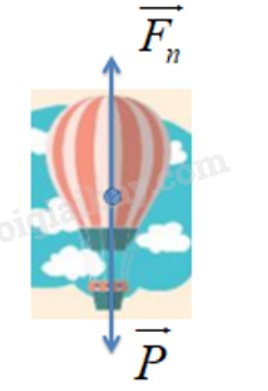
\includegraphics[scale=0.6]{../figs/VN10-2022-PH-TP020-3.jpg}
		\end{center}
	}
	\item \mkstar{2}
	
	{
		Hình biểu diễn các vecto lực tác dụng lên một máy bay đang bay ngang ở độ cao ổn định với tốc độ không đổi. Nếu khối lượng tổng cộng của máy bay là 500 tấn thì lực nâng có độ lớn bao nhiêu?
		\begin{center}
			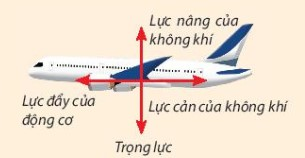
\includegraphics[scale=1]{../figs/VN10-2022-PH-TP020-2.jpg}
		\end{center}
	}
	
	\hideall{
		
		Ta có: lực nâng của không khí và trọng lực là hai lực cân bằng nên chúng có độ lớn bằng nhau.
		
		Độ lớn của lực nâng là:
		
		$$F_\text{n} = P = mg = 5\cdot 10^6\ \text{N}.$$
		
		
	}

\item \mkstar{3}


{
	Một thiết bị vũ trụ có khối lượng $\SI{70,0}{kg}$. Khi thiết bị này cất cánh từ bề mặt Mặt Trăng, lực nâng hướng thẳng đứng, lên khỏi bề mặt Mặt Trăng do động cơ tác dụng lên thiết bị là $\SI{500}{N}$. Gia tốc rơi tự do trên bề mặt Mặt Trăng là $\SI{1,6}{m/s}^2$. Hãy xác định:
	\begin{enumerate}[label=\alph*)]
		\item  Trọng lượng của thiết bị này khi ở trên Mặt Trăng.
		
		\item Tổng hợp lực nâng của động cơ và lực hấp dẫn của Mặt Trăng tác dụng lên thiết bị.
		
		\item Gia tốc của thiết bị khi cất cánh từ bề mặt Mặt Trăng.
		
	\end{enumerate}
}

\hideall
{
	\begin{enumerate}[label=\alph*)]
		\item  Trọng lượng của thiết bị này khi ở trên Mặt Trăng
		
		$$P = mg = \SI{112}{N}.$$
		
		\item Ta có:
		
		- Lực nâng của động cơ: $F_\text{n} = \SI{500}{N}.$
		
		- Lực hấp dẫn của Mặt Trăng tác dụng lên thiết bị: $P = \SI{112}{N}.$
		
		Hai lực này cùng phương, ngược chiều.
		
		- Tổng hợp lực nâng của động cơ và lực hấp dẫn của Mặt Trăng tác dụng lên thiết bị là:
		
		$$F = F_\text{n} - P = \SI{388}{N}.$$
		
		\item Gia tốc của thiết bị khi cất cánh từ bề mặt Mặt Trăng
		
		$$a = \dfrac{F}{m} = \SI{5,53}{m/s}^2.$$
		
	\end{enumerate}
}

\item \mkstar{3}\\
{Một chiếc xe ô tô có khối lượng tổng cộng người và xe là $\SI{550}{\kilogram}$ đang chuyển động trên mặt đường nằm ngang. Biết lực đẩy gây ra bởi động cơ tác dụng lên ô tô là $\SI{300}{\newton}$ và tổng lực cản của môi trường lên ô tô là $\SI{200}{\newton}$. Biểu diễn hai lực trên tác dụng lên ô tô và tính gia tốc của ô tô.

}
\hideall{
\begin{center}
	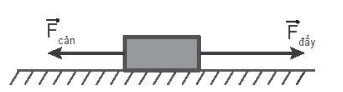
\includegraphics[width=0.4\linewidth]{../figs/VN10-2022-PH-TP020-P-2}
\end{center}
$$F=F_\text{đẩy}-F_\text{cản}=\SI{100}{\newton}$$
$$\Rightarrow a=\dfrac{F}{m}\approx\SI{0.18}{\meter/\second^2}.$$
}

\item \mkstar{3}\\
{Lực đẩy tối đa có thể tác dụng lên một chiếc xe thể thao để nó chuyển động trên mặt đường nằm ngang là $\SI{500}{\newton}$. Biết lực cản của không khí tác dụng lên xe phụ thuộc vào vận tốc $v$ theo công thức $F=0,2v^2$. Hãy xác định tốc độ tối đa của xe.

}
\hideall{
$v=\SI{50}{\meter/\second}$.
}

\item \mkstar{3}\\
{Một chiếc thuyền máy đang được lái về phía tây dọc theo một con sông. Lực đẩy gây ra bởi động cơ là $\SI{560}{\newton}$ hướng về phía tây. Lực ma sát giữa thuyền và mặt nước là $\SI{180}{\newton}$, lực cản của không khí lên thuyền là $\SI{60}{\newton}$ hướng về phía đông.
	\begin{center}
		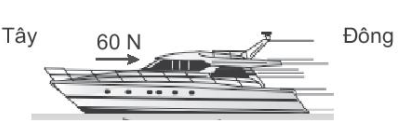
\includegraphics[width=0.4\linewidth]{../figs/VN10-2022-PH-TP020-P-3}
	\end{center}
\begin{enumerate}[label=\alph*)]
	\item Biểu diễn các lực tác dụng lên thuyền theo phương ngang.
	\item Xác định lực tổng hợp tác dụng lên thuyền máy theo phương ngang.
\end{enumerate}
}
\hideall{
\begin{enumerate}[label=\alph*)]
	\item 
	\begin{center}
		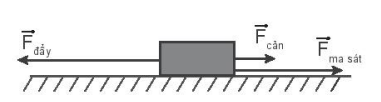
\includegraphics[width=0.4\linewidth]{../figs/VN10-2022-PH-TP020-P-4}
	\end{center}
\item $F=\SI{320}{\newton}$.
\end{enumerate}
}

\item\mkstar{4}\\
{Khi một quả cầu chuyển động trong chất lỏng, vật chịu tác dụng của lực cản được gọi là lực nội ma sát. Biểu thức độ lớn của lực nội ma sát được các định bởi định luật Stokes: $f=6\pi \cdot r\cdot v\cdot\eta$,\\
	trong đó:
	\begin{itemize}
		\item $f$ là lực nội ma sát $\left(\si{\newton}\right)$;
		\item $r$ là bán kính của quả cầu $\left(\si{\meter}\right)$;
		\item $v$ là tốc độ tức thời của quả cầu $\left(\si{\meter/\second}\right)$;
		\item $\eta$ là hệ số ma sát nhớt hay độ nhớt của chất lỏng $\left(\si{\pascal\cdot s}\right)$.
	\end{itemize}
Khi chuyển động của quả cầu đạt trạng thái ổn định, quả cầu chuyển động với tốc độ bão hoà được xác định bởi biểu thức
$$v_{bh}=\dfrac{2r^2\cdot g\cdot\left(\sigma - \rho\right)}{9\eta}$$
trong đó:
\begin{itemize}
	\item $v_{bh}$ là tốc độ bão hoà $\left(\si{\meter/\second}\right)$;
	\item $g$ là gia tốc trọng trường $\left(\si{\meter/\second^2}\right)$;
	\item $\sigma$ là khối lượng riêng của quả cầu $\left(\si{\kilogram/\meter^3}\right)$;
	\item $\rho$ là khối lượng riêng của chất lỏng $\left(\si{\kilogram/\meter^3}\right)$.
\end{itemize}
Xét một quả cầu đang rơi thẳng đều trong một chất lỏng với các thông số sau:
\begin{itemize}
	\item $\text{Đường kính của quả cầu}=\SI{3.0}{\milli\meter}$;
	\item $\text{Khối lượng riêng của quả cầu}=\SI{2500}{\kilogram/\meter^3}$;
	\item $\text{Khối lượng riêng của chất lỏng}=\SI{875}{\kilogram/\meter^3}$;
	\item $\text{Tốc độ bão hoà}=\SI{160}{\milli\meter/\second}$.
\end{itemize}
Biết gia tốc trọng trường là $\SI{9.8}{\meter/\second^2}$. Hãy xác định độ nhớt của chất lỏng và độ lớn của lực nội ma sát tác dụng lên vật đang chuyển động ở tốc độ bão hoà.
}
\hideall{
Độ nhớt của chất lỏng: 
$$\eta=\dfrac{2r^2\cdot g\cdot\left(\sigma-\rho\right)}{9v_{bh}}\approx\SI{5.0E-2}{\pascal\cdot \second}.$$
Độ lớn của lực nội ma sát tác dụng lên vật ở tốc độ bão hoà:
$$f=6\pi\cdot r\cdot v\cdot \eta =\SI{2.3E-4}{\newton}.$$
}


\end{enumerate}